\documentclass[tikz,border=5pt]{standalone}
\usepackage{luatexja}
\usepackage[hiragino-pron]{luatexja-preset}
\usepackage{amsmath,amssymb}
\usetikzlibrary{arrows.meta,patterns}

\begin{document}
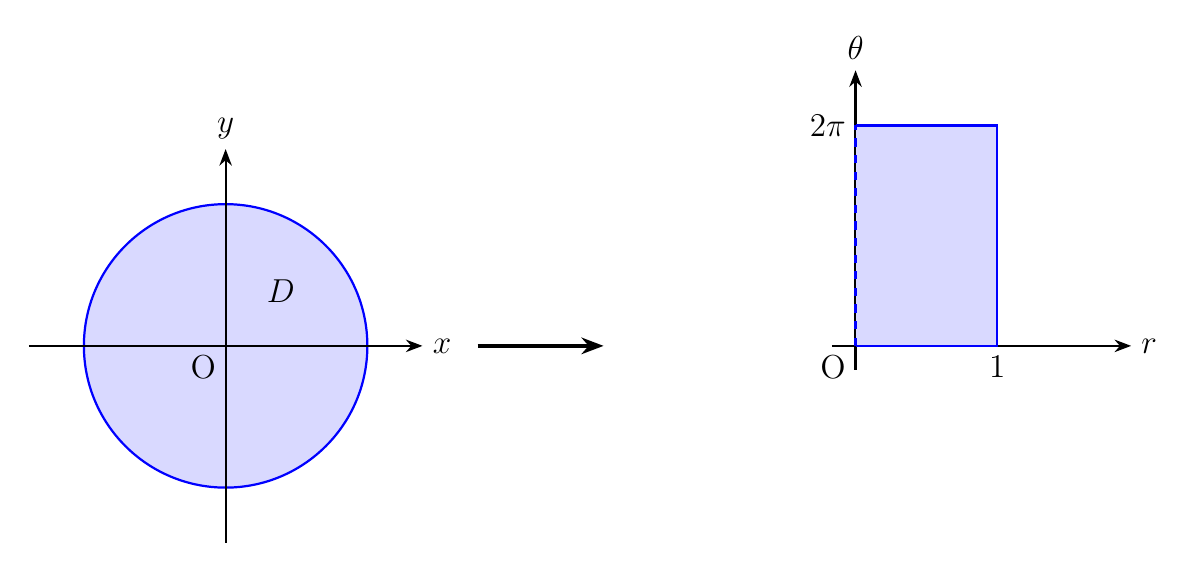
\begin{tikzpicture}[every node/.style={font=\large}]
  \begin{scope}
    % Shaded disk (behind axes)
    \fill[blue!15] (0,0) circle (1.8);
    \draw[thick, blue] (0,0) circle (1.8);

    % xy plane (on top)
    \draw[-{Stealth[length=6pt]}, thick] (-2.5,0) -- (2.5,0) node[right] {$x$};
    \draw[-{Stealth[length=6pt]}, thick] (0,-2.5) -- (0,2.5) node[above] {$y$};

    \node at (0.7,0.7) {$D$};
    \node[below left] at (0,0) {O};
  \end{scope}

  % Arrow
  \draw[-{Stealth[length=8pt]}, very thick] (3.2,0) -- (4.8,0);

  \begin{scope}[xshift=8cm]
    % r-theta plane
    \draw[-{Stealth[length=6pt]}, thick] (-0.3,0) -- (3.5,0) node[right] {$r$};
    \draw[-{Stealth[length=6pt]}, thick] (0,-0.3) -- (0,3.5) node[above] {$\theta$};

    % Shaded rectangle in r-theta
    \fill[blue!15] (0,0) rectangle (1.8,2.8);
    \draw[thick, blue] (0,0) -- (1.8,0) -- (1.8,2.8) -- (0,2.8);
    \draw[thick, blue, dashed] (0,0) -- (0,2.8);

    % Labels
    \node[below] at (1.8,0) {$1$};
    \node[left] at (0,2.8) {$2\pi$};

    \node[below left] at (0,0) {O};
  \end{scope}
\end{tikzpicture}
\end{document}
